\chapter{Transformaciones conformes}

\section{Propiedades básicas}

Sea $w = f(z)$ una función analítica en un punto $z_0$ tal que $f'(z_0) \neq 0$. Sea, además, $C$ una curva suave, que pasa por $z_0$ y tiene una representación paramétrica $z(t) = x(t) + iy(t)$, con $a \leq t\leq b$. Luego,
$$w(t) = f(z(t)), \quad a \leq t \leq b$$

es la imagen $\Gamma$ de la curva $C$, la cual es también suave. De acuerdo a la regla de la cadena,
$$w'(t) = f'(z(t)) z'(t).$$

Como $C$ es una curva suave que pasa por $z_0$, se tiene que $z'(t_0) \neq 0$, donde $z(t_0) = z_0$. Denotemos por $\theta_0 = \arg z'(t_0)$ el ángulo de inclinación del vector $z'(t_0)$. Para analizar el ángulo de inclinación del vector $w'(t_0)$, denotemos por $\psi_0 = \arg f'(z(t_0))$ y, luego por las propiedades de los argumentos de un producto, se tiene
$$\phi_0 = \arg w'(t_0) = \arg f'(z(t_0)) + \arg z'(t_0) = \theta_0 + \psi_0.$$

\begin{figure}[H]
    \centering
    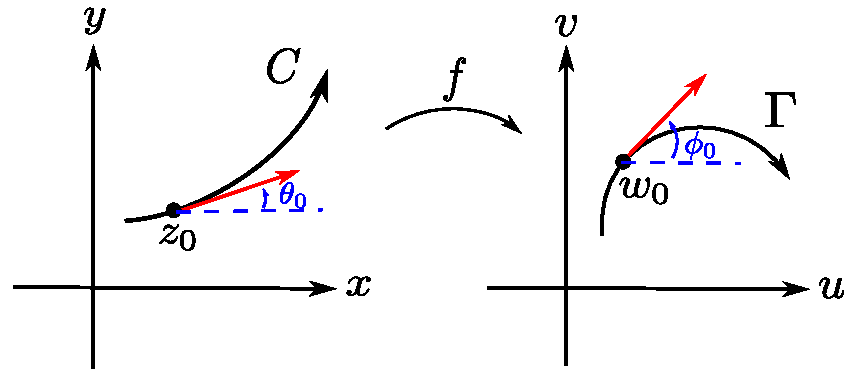
\includegraphics[scale = 0.75]{Figuras/MapeoConforme1.pdf}
    \caption{}
    \label{fig:Conforme1}
\end{figure}

En consecuencia, si $w = f(z)$ es analítica en un punto $z_0$ y $f'(z_0) \neq 0$, entonces la recta tangente a $C$ en $z_0$ es rotada en un ángulo
$$\arg f'(z(t_0))$$

por la transformación $w = f(z)$.

Supongamos, ahora, que $C_1$ y $C_2$ son dos curvas suaves que pasan por $z_0$ y con ángulos de inclinación $\theta_1$ y $\theta_2$ de las rectas tangentes, respectivamente. Entonces, por lo anterior, tenemos
\begin{align*}
    \phi_1 &= \theta_1 + \arg f'(z(t_0)) \\
    \phi_2 &= \theta_2 + \arg f'(z(t_0))
\end{align*}

y, por tanto,
$$\phi_2 - \phi_1 = \theta_2 - \theta_1,$$

es decir, el ángulo $\alpha = \phi_2 - \phi_1$ formado por $\Gamma_1$ a $\Gamma_2$ tiene igual magnitud y sentido que el ángulo $\alpha = \theta_2 - \theta_1$ formado por $C_1$ y $C_2$.

\begin{figure}[H]
    \centering
    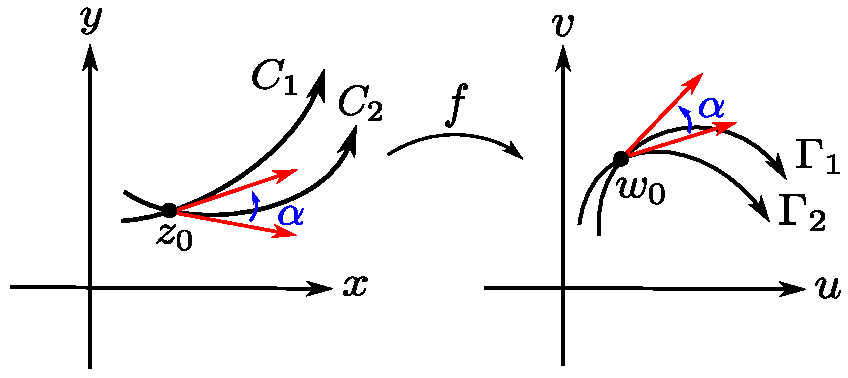
\includegraphics[scale = 0.75]{Figuras/MapeoConforme2.pdf}
    \caption{Preservación de la magnitud y el sentido del ángulo.}
    \label{fig:Conforme2}
\end{figure}

\begin{defi}
Una función que preserva magnitud y sentido de ángulos entre dos curvas suaves que pasan a través de un punto específico se dice una \textbf{aplicación conforme en tal punto}. Diremos que $f$ es, simplemente, una \textbf{aplicación conforme} si es conforme en cada punto.
\end{defi}

\begin{teorema}
Si $f$ es analítica y $f'(z) \neq 0$ para todo punto de su dominio, entonces $f$ es una aplicación conforme.
\end{teorema}

\begin{ejemplo}
Sea $D = \{z \in \mathbb{C}: Re(z) > 0, Im(z) > 0 \}$ y $F = \{z \in \mathbb{C}: Im(z) > 0\}$. La función $f: D \rightarrow F$, $f(z) = z^2$ es conformal en $D$, pues $f$ es analítica aquí y $f'(z) = 2z \neq 0$. En cambio $g: \mathbb{C} \rightarrow \mathbb{C}$, $g(z) = z^2$ no es conforme en $z_0 = 0$, ya que el ángulo que forman los ejes coordenados es $\pi/2$, en cambio, en sus imágenes forman un ángulo $\pi$. Justamente, $g'(0) = 0$.
\end{ejemplo}

\begin{propo}
Si $f$ es una transformación conforme, analítica en su dominio y biyectiva, entonces $f^{-1}$ es también conforme.
\end{propo}

\begin{proof}
La inversa es también analítica y
$$\left( f^{-1}\right)'(w) = \frac{1}{f'(z)} \neq 0,$$

donde $f(z) = w$.
\end{proof}

\begin{propo}
Si $f$ y $g$ son funciones analíticas tales que $g \circ f$ existe, $f'(z_0) \neq 0$ y $g'(f(z_0)) \neq 0$, entonces $g \circ f$ es conformal en $z_0$.
\end{propo}

\begin{proof}
Por la regla de la cadena, la compuesta $g \circ f$ es analítica y
$$(g\circ f) (z_0) = g'(f(z_0)) f'(z_0) \neq 0.$$

Probando así el teorema.

\end{proof}

Dado dos dominios $D$ y $E$, ¿será posible tener una aplicación conforme $f: D \rightarrow E$? La respuesta es positiva, pero la demostración requiere mayores resultados que se escapan del curso.

\begin{teorema}[de la aplicación de Riemann] \label{RiemannMap}
Sea $D$ una región simplemente conexa tal que $D \neq \mathbb{C}$. Entonces, existe una aplicación conforme biyectiva $f: D \rightarrow B$ donde $B = \{z \in \mathbb{C} : |z| < 1\}$. Más aún, para algún $z_0 \in D$ fijo, podemos encontrar una función $f$ tal que $f(z_0) = 0$ y $f'(z_0) > 0$. Con tal especificación, $f$ es única.
\end{teorema}

Asumiendo el teorema de la aplicación de Riemann, es posible dar respuesta a la pregunta mencionada arriba.

\begin{propo}
Sean $D$ y $E$ dos regiones simplemente conexas con $D \neq \mathbb{C}$ y $E \neq \mathbb{C}$, entonces existe una aplicación conforme biyectiva $g: D \rightarrow E$. 
\end{propo}

\begin{proof}
Por el teorema de la aplicación de Riemann, existen dos aplicaciones conformes biyectivas $f: D \rightarrow B$ y $h: E \rightarrow B$. Definiendo $g = h^{-1} \circ f$, se tiene la proposición.

\begin{figure}[H]
    \centering
    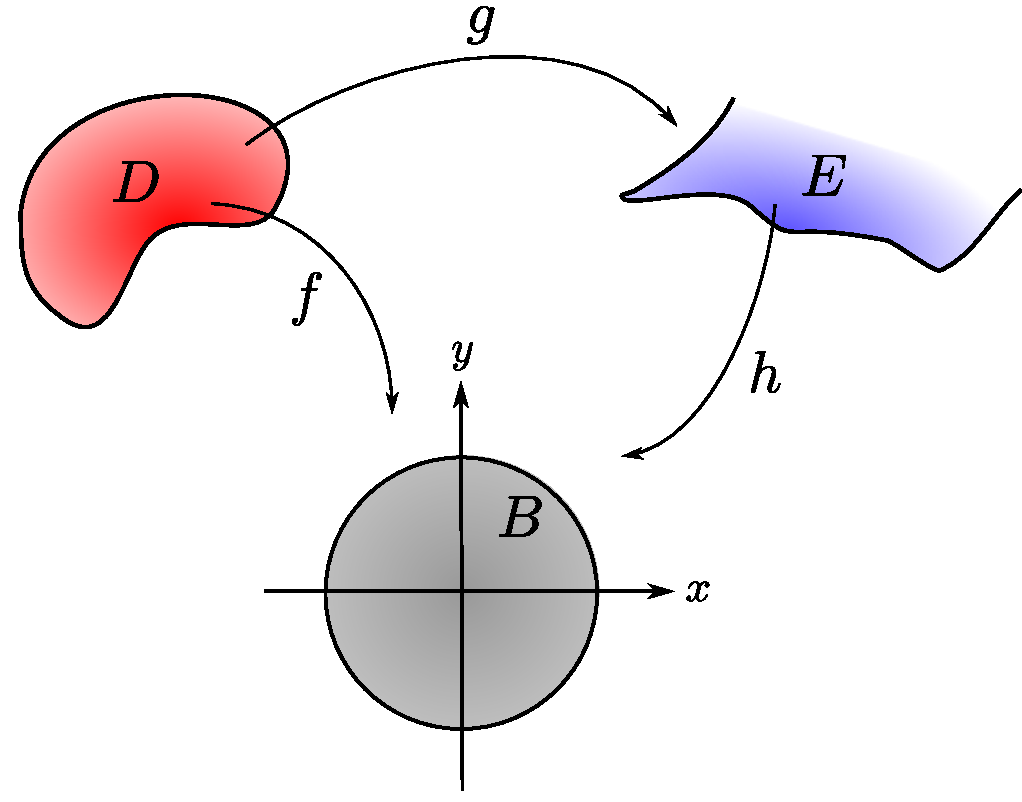
\includegraphics[scale = 0.5]{Figuras/MapeoConforme3.pdf}
    \caption{Aplicación entre dos regiones simplemente conexas.}
    \label{fig:Conforme3}
\end{figure}
\end{proof}

\begin{lema}[de Schwarz]
Sea $f(z)$ una función analítica en  $D = \{z \in \mathbb{C}: |z| < 1 \}$, y $f(0) = 0$, $|f(z)| \leq 1$. Entonces, 
\begin{equation}
 \forall z \in D:~ |f(z)| \leq |z|   \label{LemaSchawarz1}
\end{equation}

y
\begin{equation}
 |f'(0)| \leq 1. \label{LemaSchawarz2}
\end{equation}

La igualdad \eqref{LemaSchawarz1} ocurre en algún punto $0 \neq z \in D$ si y sólo si $f(z) =  \alpha z$, donde $\alpha \in \mathbb{C}$ tal que $|\alpha| = 1$.
\end{lema}
\begin{proof}

Sea 
$$g(z) = \left\{ \begin{array}{cl}
    \frac{f(z)}{z}, & \mbox{si}~ z\neq 0  \\
    f'(0), & \mbox{si}~ z = 0 
\end{array} \right. .$$

Probemos que $g$ es analítica en $D$. Como $f$ es analítica para  $|z| < 1$ y $f(0) = 0$, podemos escribir $f$ como la siguiente serie de potencias
$$f(z) = a_1z + a_2 z^2 + \cdots = \sum_{n=1}^{\infty} a_n z^n, \quad |z| < 1 $$

donde se hizo $a_0 = f(0) = 0$. Luego,
$$\frac{f(z)}{z} = a_1 + a_2 z + a_3 z^2 + \cdots = \sum_{n=0}^{\infty} a_{n+1} z^n.$$

Entonces, $z = 0$ es una singularidad removible de $f(z)/z$, así definiendo la función en $z = 0$ como $a_1 = f'(0)$, la función resultante es $g$, la cual es analítica en todo $D$. 

Sea $D_r = \{z \in \mathbb{C} : |z| \leq r\}$ para $0 <r <1$. Entonces, $g$ es analítica en $D_r$, y en $|z| = r$, se cumple que
$$|g(z)| = \left| \frac{f(z)}{z} \right| \leq \frac{1}{r}.$$

Por el teorema del módulo máximo,
$$\forall z \in D_r: ~ |g(z)| \leq \frac{1}{r} \Rightarrow |f(z)| \leq \frac{|z|}{r}.$$

Si mantenemos $z \in D$ fijo, podemos tomar  $r \to 1$ para sí obtener
$$|f(z)| \leq |z|.$$

Claramente, $|g(0)| \leq 1$, ésto es, $|f'(0)| \leq 1$.

Finalmente, si $|f(z_0)/z_0| = 1$ para algún $z_0 \neq 0$ en el disco unitario, entonces, por el teorema del módulo máximo, $f(z)/z$ no puede tener un máximo a menos que sea constante, así existe una constante $\alpha$ con $|\alpha| = 1$ tal que $f(z)/z = \alpha.$

\end{proof}

\subsection*{Prueba de la unicidad del teorema \ref{RiemannMap}*}

\begin{proof}
Supongamos que $f$ y $g$ son mapeos conformes biyectivos de $D$ sobre $B$, con $f(z_0) = g(z_0) = 0$, $f'(z_0) > 0$ y $g'(z_0) > 0$. Queremos mostrar que $f(z) = g(z)$ para todo $z \in D$. Para hacer ésto, definamos $h: B \rightarrow B$, $h(w) = g(f^{-1}(w))$, la cual es analítica en $B(0,1)$ y $h(0) = g(f^{-1}(0)) = g(z_0) = 0$. Por el lema de Schwarz, $|h(w)|\leq |w|$ para todo $w \in B$. Exactamente el mismo argumento se aplica a $h^{-1} = f \circ g^{-1}$, así que $|h^{-1}(\xi)| \leq |\xi|$ para todo $\xi \in D$. Con $\xi = h(w)$ esto da $|w| \leq h(w)$. Al combinar estas desigualdades, obtenemos $|h(w)| = w$ para todo $w\in B$. El lema de Schwarz nos dice ahora que $h(w) = \alpha w$ para un $\alpha \in \mathbb{C}$, con $|\alpha| = 1$. Así, $\alpha w = g(f^{-1}(w))$. Con $z = f^{-1}(w)$ obtenemos $\alpha f(z) = g(z)$ para todo $z\in D$. En particular, $\alpha f'(z_0) = g'(z_0)$. Ya que tanto $f'(z_0)$ como $g'(z_0)$ son números reales positivos, también lo es $\alpha$. Así, $\alpha = 1$ y, por tanto, $f(z) = g(z)$, como se quería.
\end{proof}

\section{Transformaciones de Möbius}

Un ejemplo importante de aplicaciones conformes son las \textbf{transformaciones fraccionales lineales} o \textbf{de Möbius}:
$$T(z) = \frac{az+b}{cz+d}, \quad z \neq - \frac{d}{c},$$

con $ad-bc \neq 0$. En efecto,
$$T\,'(z) = \frac{ad-bc}{(cz+d)^2} \neq 0.$$

Luego, $T$ es una aplicación conforme en cada $z\in \mathbb{C} \setminus \left\{-\frac{d}{c} \right\}$.

Son biyectivas en $\mathbb{C}\setminus \left\{-\frac{d}{c} \right\}$ sobre $\mathbb{C}\setminus \left\{\frac{a}{c} \right\}$ y, por tanto, su inversa
$$T^{-1}(w) = \frac{(-d)w + b}{cw-a}$$

es también conforme.

Notar que $T = T_4 \circ T_3 \circ T_2 \circ T_1$, donde 
\begin{align*}
    T_1(z) &= z + \frac{d}{c}; \quad T_2(z) = \frac{1}{z}; \\
    T_3(z) &= \frac{bc-ad}{c^2}z; \quad  T_4(z) = z+ \frac{a}{c}.
\end{align*}

\begin{ejemplo}
Dada la transformación de Möbius
$$T(z) = \frac{az+b}{cz+d}.$$

Si $a = 1$, $c = 0$ y $d = 1$, obtenemos $T(z) = z+b$, la cual es una traslación de los puntos en el plano complejo de acuerdo al vector $b$.

Si $b = c = 0$ y $d = 1$, obtenemos $T(z) = az$, la cual es una rotación por $\arg(a)$ y una amplificación por $|a|$.

Finalmente, si $a = d = 0$ y $b = c = 1$, obtenemos $T(z) = 1/z$, la cual es una inversión donde envía a todo $z = r e^{i\theta}$ a $z^{-1} = \overline{z}/|z|^2 = r^{-1}  e^{-i\theta}$.
\end{ejemplo}

\textbf{Observaciones:}

\begin{enumerate}
    \item La composición de dos transformaciones de Möbius es una transformación de Möbius (ejercicio para el lector).
    
    \item Sea
    $$T(z) = \frac{az+b}{cz+d}; \quad z \neq - \frac{d}{c}$$
    
    una transformación de Möbius. Notar que
    $$\frac{(\lambda a) z + \lambda b}{(\lambda c)z + \lambda d} = \frac{az + b}{cz+d},$$
    
    es decir, los coeficientes $a, b, c, d$ no son únicos.
    
    \item Por otro lado, podemos extender una transformación de Möbius al plano extendido $\overline{\mathbb{C}}$ como sigue:
    $$T(z) = \left\{ \begin{array}{cl}
        \frac{az+b}{cz+d}, & \mbox{si}~ z \neq - \frac{d}{c}, \infty  \\
        \frac{a}{c}, &  \mbox{si}~ z = \infty \\
        \infty, & \mbox{si}~ z = - \frac{d}{c}
    \end{array} \right. .$$
\end{enumerate}    

\begin{propo}
Cualquier mapeo conforme de $D = \{z \in \mathbb{C}: |z| < 1\}$ sobre si mismo es una transformación fraccional lineal de la forma
$$T(z) = e^{i\theta} \frac{z-z_0}{1-\overline{z_0} z}$$

para algún $z_0 \in D$ fijo y $\theta \in [0,2\pi[$; más aún, cualquier $T$ de esta forma es un mapeo conforme de $D$ sobre $D$.
\end{propo}

\begin{proof}
Primero verifiquemos que para $T$ de esta forma, $|z| = 1$ implica que $|T(z)| = 1$. En efecto,
$$|T(z)| = \left|\frac{z-z_0}{1-\overline{z_0} z} \right| = \frac{|z-z_0|}{|z| \,|z^{-1} - \overline{z_0}|}.$$

Pero $|z| = 1$ y, por tanto, $z^{-1} = \overline{z}$. Así, obtenemos
$$|T(z)|= \frac{|z-z_0|}{|\overline{z} - \overline{z_0}|} = \frac{|z-z_0|}{|\,\overline{z-z_0}\,|} = 1.$$

La única singularidad de $T$ está en $z = \overline{z_0}^{-1}$, que está fuera del círculo unitario, pues
$$|z| = \left|\frac{z_0}{z_0 \overline{z_0}} \right| = \frac{|z_0|}{|z_0|^2} = \frac{1}{|z_0|} \geq 1.$$

Entonces, por el teorema del módulo máximo, $|T(z)| \leq 1$ para todo $z \in D$, es decir, $T$ transforma $D$ en $D$ (no sobre a priori). Pero su inversa,
$$T^{-1}(w) = e^{-i\theta} \left[\frac{w - (-e^{i\theta}z_0)}{1-(-e^{-i\theta} \overline{z_0})w} \right],$$

la cual, puesto que tiene la misma forma que $T$, es también un mapeo de $D$ en $D$. Así que $T$ es conforme de $D$ sobre $D$.

Sea $R: D \rightarrow D$ cualquier mapeo conforme. Sea $z_0 = R^{-1}(0)$ y sea $\theta = \arg R'(z_0)$. El mapeo $T$ definido, también tiene $T(z_0) = 0$ y  $\theta = \arg T'(z_0)$. En efecto,
$$T\,'(z) = e^{i\theta} \left[ \frac{1-|z_0|^{2}}{(1-\overline{z_0} z)^2} \right]$$

el cual, en $z = z_0$, es igual a
$$e^{i\theta} \left(\frac{1}{1-|z_0|^2} \right)$$

una constante real por $e^{i\theta}$. Así, por la unicidad de los mapeos conformes, $R = T$.
\end{proof}

Este resultado nos dice que la única forma de transformar un disco sobre sí mismo conformemente, es por medio de una transformación fraccional lineal. Estas transformaciones poseen otras propiedades adicionales, como se mostrará en los siguientes resultados.

\begin{propo}
Sea $T$ una transformación fraccional lineal. Si $L \subset \mathbb{C}$ es una línea recta y $S \subset \mathbb{C}$ es una circunferencia, entonces $T(L)$ es una línea recta o una circunferencia, y $T(S)$ es una línea recta o una circunferencia.
\end{propo}

\begin{proof}
Escribamos $T = T_4 \circ T_3 \circ T_2 \circ T_1$, donde 
\begin{align*}
    T_1(z) &= z + \frac{d}{c}; \quad T_2(z) = \frac{1}{z}; \\
    T_3(z) &= \frac{bc-ad}{c^2}z; \quad T_4(z) = z+ \frac{a}{c}.
\end{align*}

Es claro que $T_1$, $T_3$ y $T_4$ transforman líneas en líneas, y circunferencias en circunferencias. Así que si podemos verificar la conclusión para $T(z) = 1/z$, la demostración estará completa. Asumamos primero que $S: |z-z_0| = r$ y sea
$$f(S) = \left\{ w = \frac{1}{z} : z \in S\right\}.$$

Escribamos $S$ de la forma
$$(z-z_0)(\overline{z} - \overline{z_0}) = r^2,$$

tenemos
$$z \overline{z} - z_0 \overline{z} - \overline{z_0} z = r^2 - |z_0|^2$$

o, en términos de $w$,
\begin{equation}
\frac{1}{w \overline{w}} - \frac{z_0}{\overline{w}} - \frac{\overline{z_0}}{w} = r^2-|z_0|^2.    \label{Mobius1}
\end{equation}

Si $r = |z_0|$, es decir, si $S$ pasa a través del origen, \eqref{Mobius1} es equivalente a 
$$1- z_0 w - \overline{z_0} \overline{w} = 0 \Rightarrow Re(z_0 w) = \frac{1}{2}.$$

En ese caso, si $z_0 = x_0 + iy_0$ y $w = u+iv$, la ecuación se convierte en
$$ux_0 - vy_0 = \frac{1}{2},$$

ésto es, $f(S)$ es una línea en el plano $uv$.

Por otro lado, si $r \neq |z_0|$, entonces \eqref{Mobius1} es equivalente a
$$w \overline{w} - \left( \frac{\overline{z_0}}{|\overline{z_0}|^2 -r^2} \right) \overline{w} - \left( \frac{z_0}{|\overline{z_0}|^2 -r^2} \right) w = - \frac{1}{|z_0|^2 -r^2},$$

definiendo $\beta = \overline{z_0}/(|\overline{z_0}|^2 -r^2)$, obtenemos
$$w \overline{w} - \beta \overline{w} - \overline{\beta} w + |\beta|^2 = \frac{r^2}{(|z_0|^{2} - r^2)^2}.$$

Por lo tanto,
$$|w - \beta|^2 = \left(\frac{r}{|z_0|^{2} - r^2} \right)^2,$$

es decir, $f(S)$ es una circunferencia con centro $\beta$ y radio $|r/(|z_0|^2-r^2)|$.

Finalmente, para la línea recta $L$, tenemos que si $z = x+iy \in L$, entonces existen $a,b,c \in \mathbb{R}$, no todos nulos, tales que
$$ax+by = c.$$

Haciendo $z_0 = a-bi$, 
$$Re(z_0 z) = c \Rightarrow z_0 z + \overline{z_0} \overline{z} = 2c.$$

Se sigue, como lo desarrollado previamente, que $f(L)$ es o una circunferencia o una línea.

 \end{proof}

\begin{propo}
Si $z_1, z_2, z_3, w_1, w_2, w_3 \in \mathbb{C}$ tales que $z_i \neq z_j$ y $w_i \neq w_j$ para $i \neq j$, entonces existe una única transformación de Möbius que lleva $z_i \to w_i$
\end{propo}

\begin{proof}
Para $z,w \in \mathbb{C}$, se define la ecuación
\begin{equation}
 \frac{w-w_1}{w-w_2} \frac{w_3-w_2}{w_3-w_1} = \frac{z-z_1}{z-z_2} \frac{z_3 - z_2}{z_3 - z_1}.  \label{Mobius1} 
\end{equation}

donde su solución $w = T(z)$  es una transformación de Möbius. En efecto, notemos que cada lado de la ecuación \eqref{Mobius1} es una transformación de Möbius, entonces si definimos
$$R(w) =  \frac{w-w_1}{w-w_2} \frac{w_3-w_2}{w_3-w_1}, \quad S(z) = \frac{z-z_1}{z-z_2} \frac{z_3 - z_2}{z_3 - z_1},$$

dos transformaciones de Möbius, tenemos que son invertibles. Luego,
$$R(w) = S(z) \Rightarrow w = R^{-1}(S(z)) = T(z),$$

donde $T = R^{-1} \circ S$.

Además, $T(z_i) = w_i$. Por tanto, nos queda por demostrar que es única. Para ello, utilizaremos la definición de la transformación de Möbius $S(z)$, la cual manda $z_1$ a 0, $z_3$ a 1, y $z_2$ a $\infty$ ($z_2$ es la singularidad de $S$). Sea $F$ cualquier otra transformación de Möbius,
$$F(z) = \frac{az + b}{cz + d}$$

con $R(z_1) = 0$, $R(z_3) = 1$ y $R(z_2) = \infty$ (ésto es, $c z_2 + d = 0$). Entonces, $az_1 + b = 0$, $c z_2 + d = 0$ y $(az_3 + b)/(cz_3+d) = 1$. De este modo, obtenemos que $a = -b/z_1$ y $c = -d/z_2$, así que la última condición da $b(z_1-z_3)/z_1 = d(z_2-z_3)/z_2$. Al sustituir en $F$, vemos que $F = S$.

Usemos este resultado para probar que $T$ es única. Sea $T$ cualquier transformación de Möbius que manda $z_i$ a $w_i$, $i = 1,2,3$. La transformación de Möbius $S\circ T^{-1}$ manda $w_1 = T(z_1)$ a 0, $w_3 = T(z_3)$ a 1, y $w_2 = T(z_2)$ a $\infty$. Por lo tanto, $ST^{-1}$ está determinado de esta manera única, por los cálculos precedentes. Así, $T$ está determinada de manera única, ya que $T = (S \circ T^{-1})^{-1} \circ S.$

\end{proof}

Se sigue que podemos usar una transformación de Möbius para mapear cualesquiera tres puntos en otros tres. Tres puntos están en una única circunferencia o línea, la transformación manda la circunferencia (o línea) a través de $z_1, z_2,z_3$, en la circunferencia (o línea) que pasa por $w_1, w_2, w_3$. El interior del disco se mapea a uno o dos semi-planos. Para determinar cuales, uno puede verificar donde el centro se mapea (o cualquier otro punto).

\newpage
\textbf{Observación:} Un \textbf{punto fijo} de una transformación $T$ es un $z_0$ tal que $T(z_0) = z_0$. Una transformación de Möbius distinta de la identidad tiene, a lo más, dos puntos fijos. En efecto,
    $$T(z) = z \Rightarrow \frac{az+b}{cz+d} = z \Rightarrow cz^2 + (d-a) z - b = 0.$$
    
    Notar que si $T$ tiene más de tres puntos fijos, entonces $T = Id$. Para probar ésto, usar
    $$\frac{w-w_1}{w-w_2} \frac{w_3-w_2}{w_3-w_1} = \frac{z-z_1}{z-z_2} \frac{z_3 - z_2}{z_3 - z_1}.$$

\section{Ejemplos de mapeos conformes}

Algunas transformaciones más comunes están representadas en las figuras \ref{fig:EjMapeosConformes1}, \ref{fig:EjMapeosConformes2} y \ref{fig:EjMapeosConformes3}.

\begin{ejemplo}
Encuentre un mapeo conforme que lleve al conjunto
$$A = \{z \in \mathbb{C} : 0 < \arg(z) < \pi/2, 0 < |z| < 1 \}$$

al conjunto
$$D = \{ z \in \mathbb{C} : |z| < 1\}.$$

\textbf{Solución:} En un principio uno está tentado a efectuar la transformación $z \mapsto z^4$ de tal forma que se complete el disco, sin embargo, esta transformación no mapea $A$ sobre $D$, pues omite el semieje real positivo.

Primero, consideremos $z \mapsto z^2$. Ésto mapea $A$ sobre $B = \{z \in \mathbb{C}: 0 < \arg(z) < \pi, 0 < |z| < 1\}$. Consultando a la figura \ref{fig:EjMapeosConformes1} (iv), mapeamos $B$ al primer cuadrante por $z \mapsto (1+z)/(1-z)$ y al elevar al cuadrado de nuevo, obtenemos el semiplano superior. Finalmente, usamos la transformación $z \mapsto (z-i)/(z+i)$ para así llegar al disco abierto unitario $D$.

\begin{figure}[H]
    \centering
    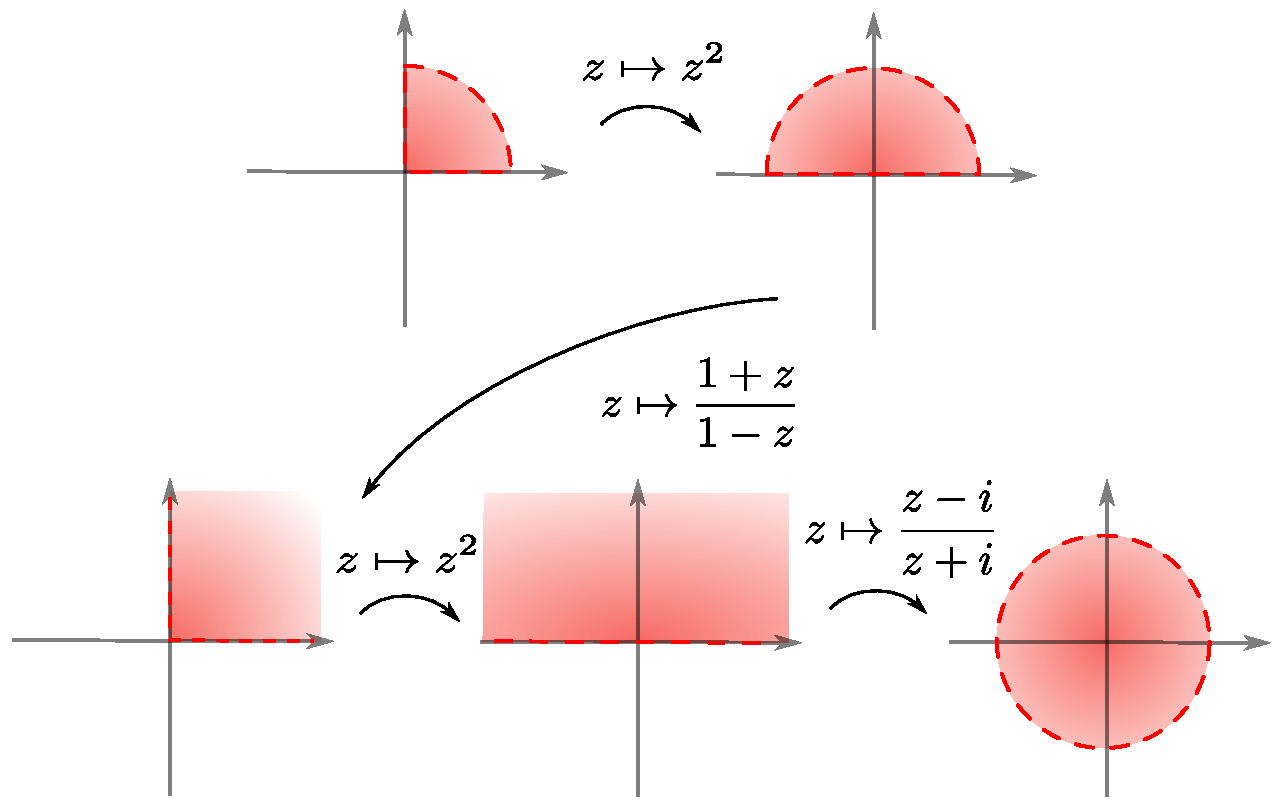
\includegraphics[scale = 0.6]{Figuras/MapeoConforme7.pdf}
    \caption{Sucesión de transformaciones que manda al cuarto de disco abierto al disco completo.}
    \label{fig:EjMapConformal}
\end{figure}

Por lo tanto, obtenemos nuestro mapeo conforme al hacer la sucesiva sustitución:
\begin{align*}
    w_1 &= z^2, \\
    w_2 &= \frac{1 + w_1}{1-w_1} = \frac{1+z^2}{1-z^2}, \\
    w_3 &= w_2^2 = \left( \frac{1+z^2}{1-z^2}\right)^2, \\
    w_4 &= \frac{w_3-i}{w_3 + i} = \frac{\left( \frac{1+z^2}{1-z^2}\right)^2 - i}{\left( \frac{1+z^2}{1-z^2}\right)^2+i}.
\end{align*}

Entonces,
$$f(z) = \frac{(1+z^2)^2 - i (1-z^2)^2}{(1+z^2)^2 + i (1-z^2)^2}.$$
\end{ejemplo}

\begin{ejemplo}
Estudie la acción de la función
$$f(z) = \frac{z-1}{z-3}$$

en la circunferencia unitaria $C$, el disco unitario $B$ y el eje real.
\\

\textbf{Solución:} Primero evaluemos $f$ en los puntos de la circunferencia $1$, $i$ y $-1$:
$$f(1) = 0, ~ f(i) = \frac{2}{5}-\frac{1}{5}i, ~ f(-1) = \frac{1}{2}.$$

Claramente las imágenes de $f$ no pertenece a una recta, por lo tanto la transformación de Möbius mapea la circunferencia unitaria en la circunferencia que pasa por $0$, $\frac{2}{5}-\frac{1}{5}i$ y $\frac{1}{2}$. 

Ahora, si evaluamos $f$ en un punto del disco unitario, como $z = 0$, $f(0) = 1/3$, la cual está en el interior de la circunferencia imagen. Entonces, $f$ mapea el disco unitario a otro disco cuya frontera es la circunferencia imagen.

Claramente $f$ manda al eje real sobre el eje real, pues la recta que pasa por $-1$, $0$ y $1$, va a la recta que pasa por $1/2$, $1/3$ y $0$. Ésto nos permitirá saber con precisión la circunferencia imagen. Aunque con los tres puntos podemos saber con precisión la ecuación de la circunferencia \footnote{La ecuación general de una circunferencia es $x^2 + y^2 + Ax + By + C = 0$ con $A,B,C \in \mathbb{R}$ no todos nulos}, usaremos el hecho de que $f$ es una transformación conforme. La curva $C$ cruza el eje real en ángulo recto en $\pm 1$ y, por ende, $f(C)$ debe cruzar el eje real también en ángulo recto, en $0$ y $1/2$. Entonces, $f(C)$ es la circunferencia de radio $1/4$ con centro $1/4$.
\end{ejemplo}

\newpage

\begin{figure}[H]
    \centering
    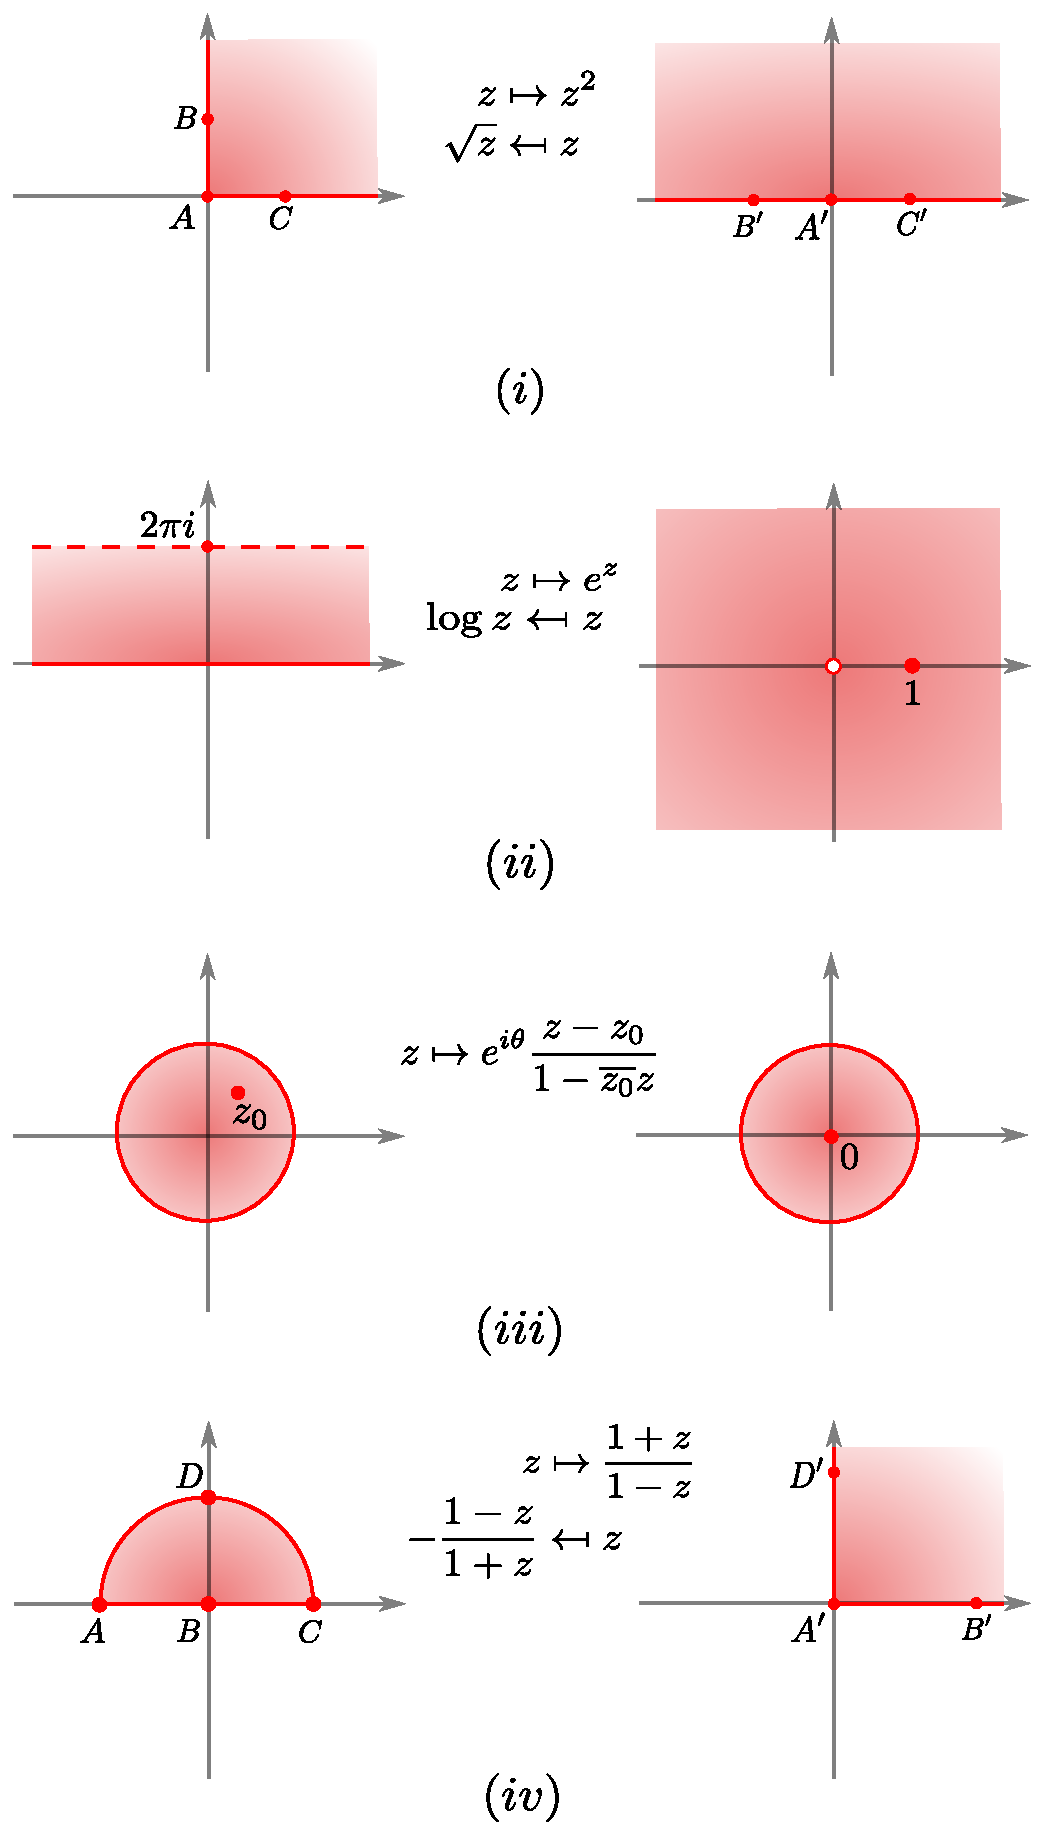
\includegraphics[scale = 0.7]{Figuras/MapeoConforme4.pdf}
    \caption{Transformaciones comunes parte 1.}
    \label{fig:EjMapeosConformes1}
\end{figure}

\begin{figure}[H]
    \centering
    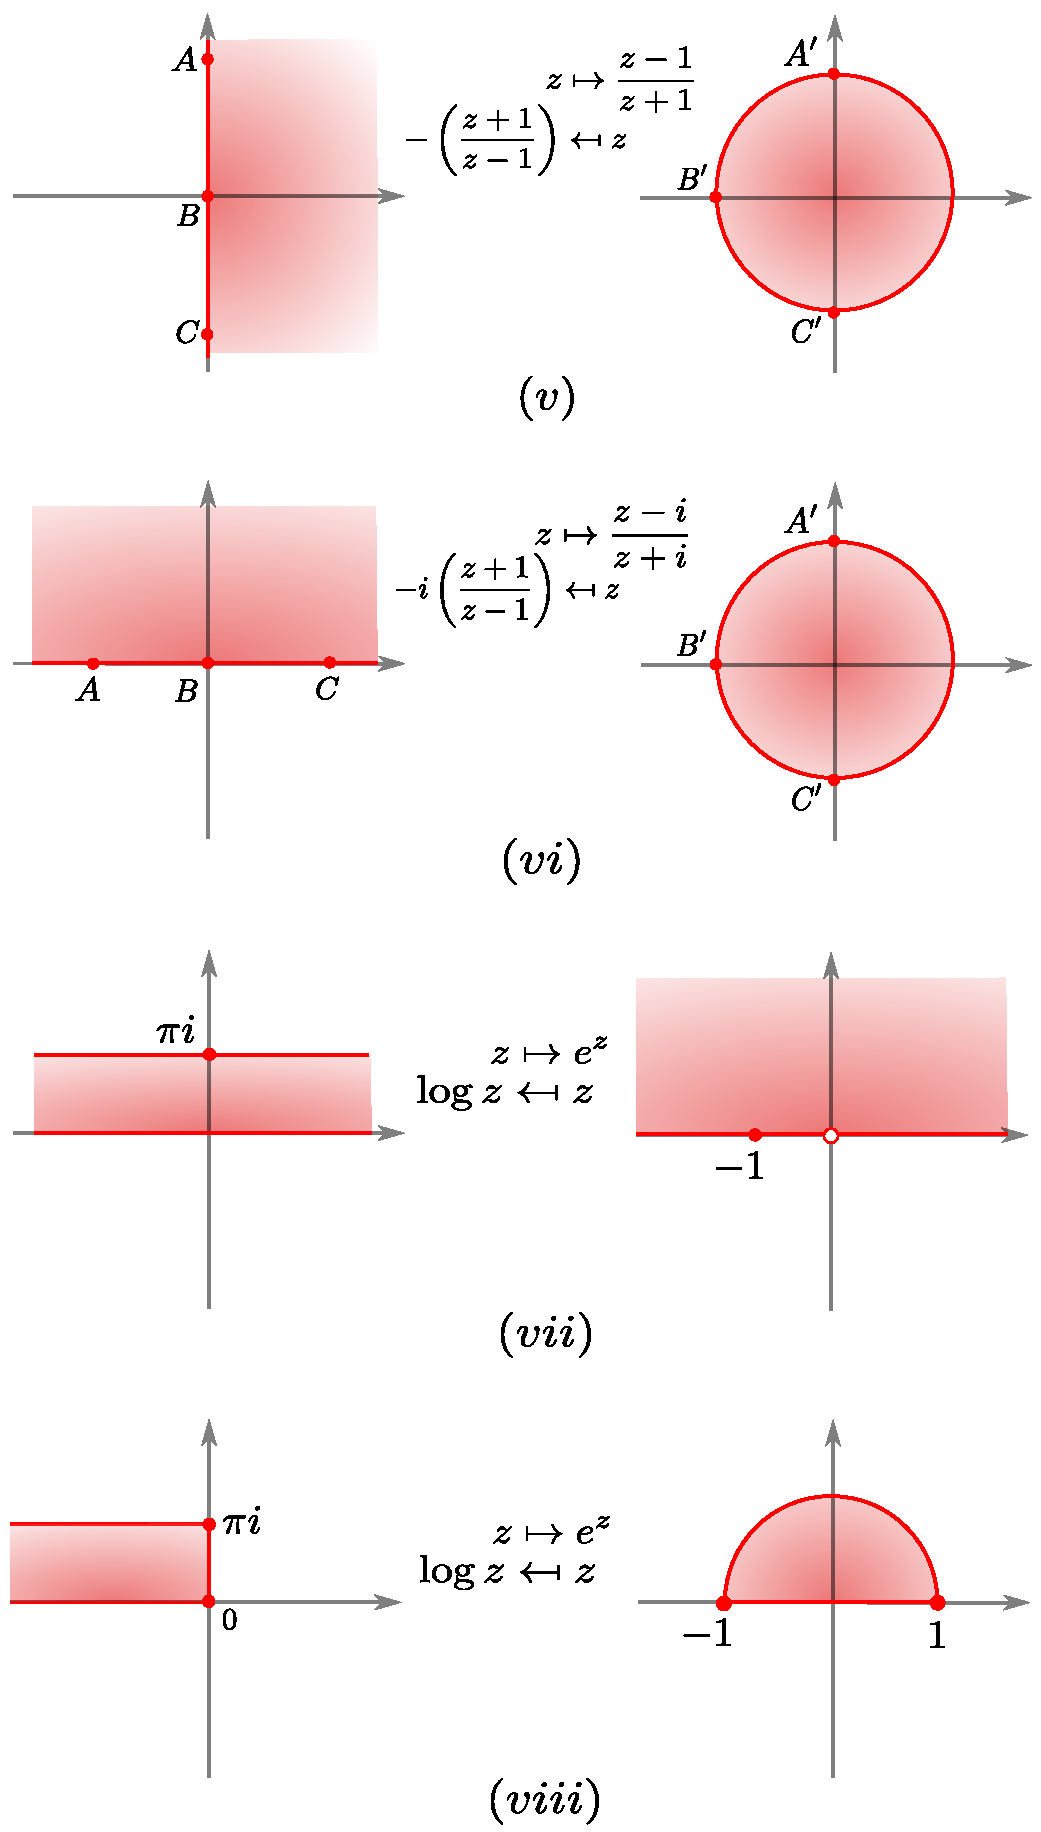
\includegraphics[scale = 0.7]{Figuras/MapeoConforme5.pdf}
    \caption{Transformaciones comunes parte 2.}
    \label{fig:EjMapeosConformes2}
\end{figure}

\begin{figure}[H]
    \centering
    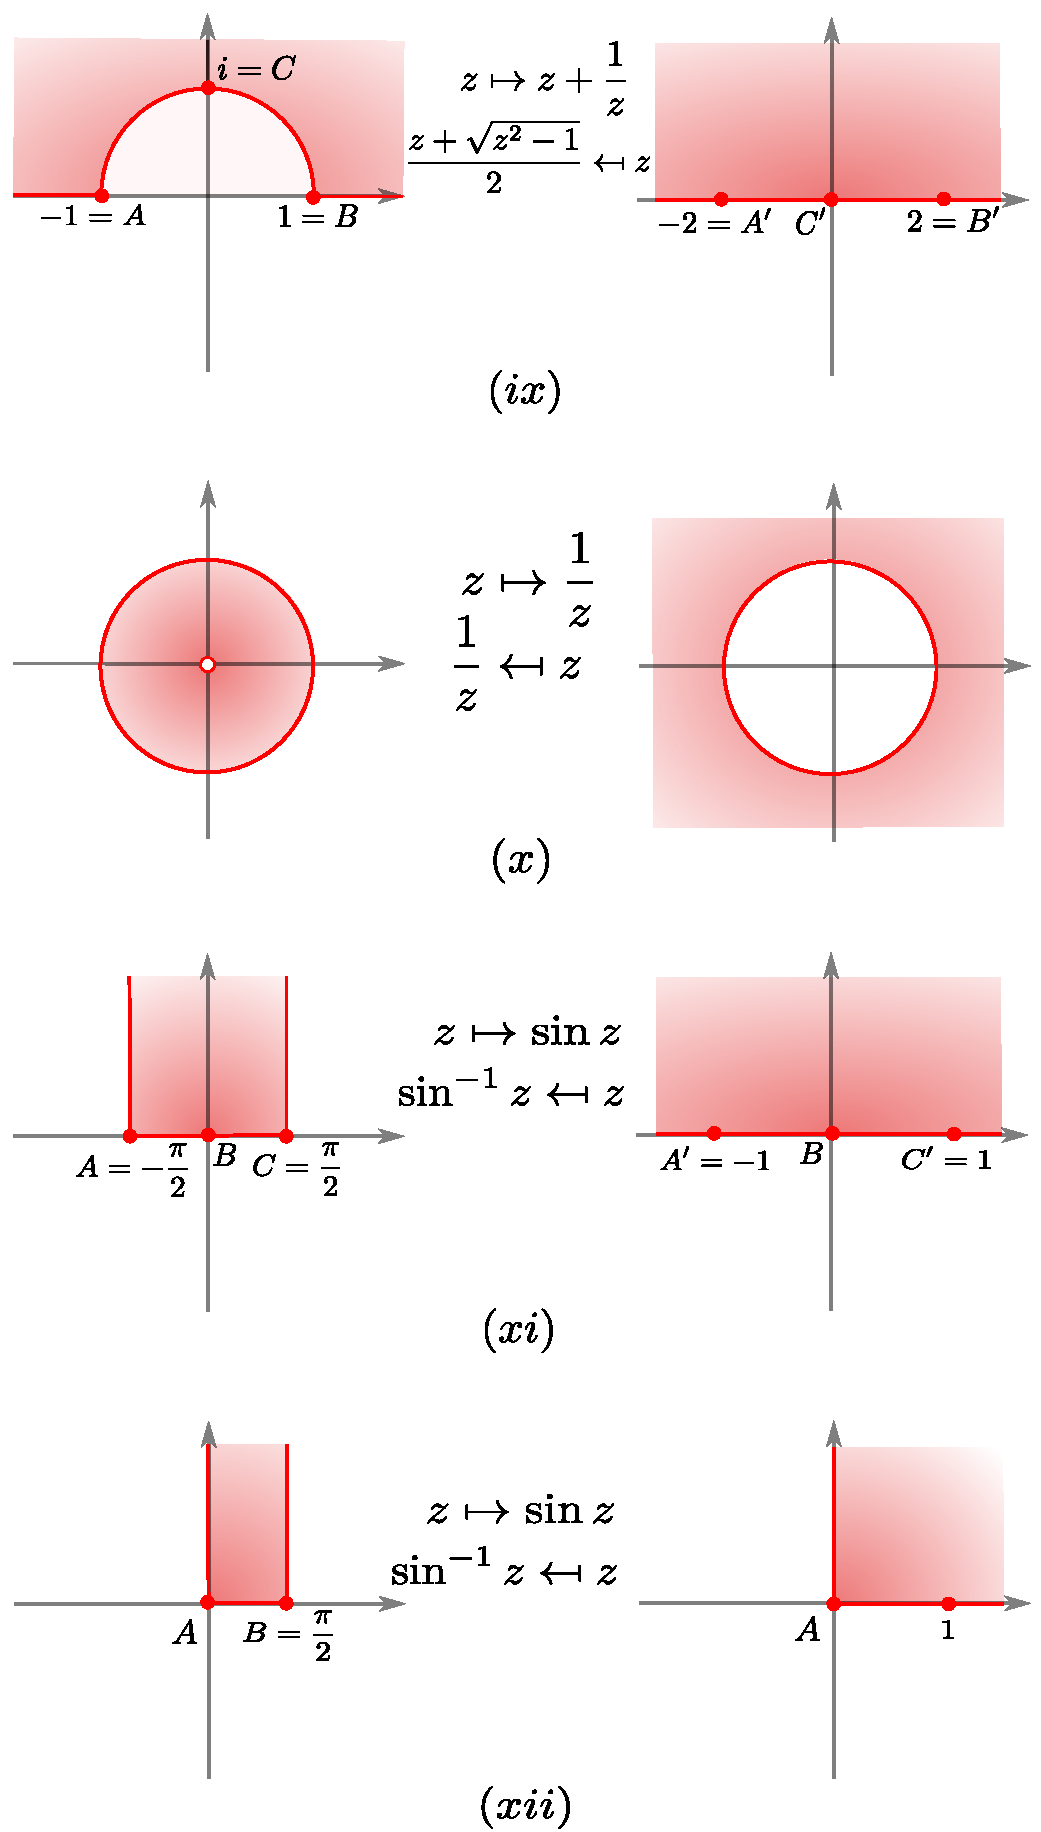
\includegraphics[scale = 0.7]{Figuras/MapeoConforme6.pdf}
    \caption{Transformaciones comunes parte 3.}
    \label{fig:EjMapeosConformes3}
\end{figure}

%\section{Aplicaciones Físicas}\subsection{Problema de Dirichlet y Neumann}\subsection{Conducción de calor}\subsection{Electrostática}\subsection{Hidrodinámica}




